The goal of the design of cloud deployments was to be cloud agnostic, meaning it should work with any cloud provider with minimal/no changes. For that reason, all services are meant to be deployed in a Kubernetes cluster, but the location or structure of the cluster doesn't matter. All of the biggest cloud providers have Kubernetes as a Service (KaaS) offering moreover it is very common along smaller providers as well.

The overall design of the cloud services can be seen in figure \ref{fig:cloud_services}. Services are communicating with each other in two ways:
\begin{itemize}
    \item Via Cloud broker - Backend and Cloud-Agent are both subscribed to a series of topics and exchange information through MQTT messages sent to the cloud broker. 
    \item Via REST endpoints - Backend services expose the REST endpoint which is consumed by Frontend. Frontend itself is only meant to serve HTML documents and be a consumer of the backend endpoint.
\end{itemize}

\begin{figure}[H]
    \centering
    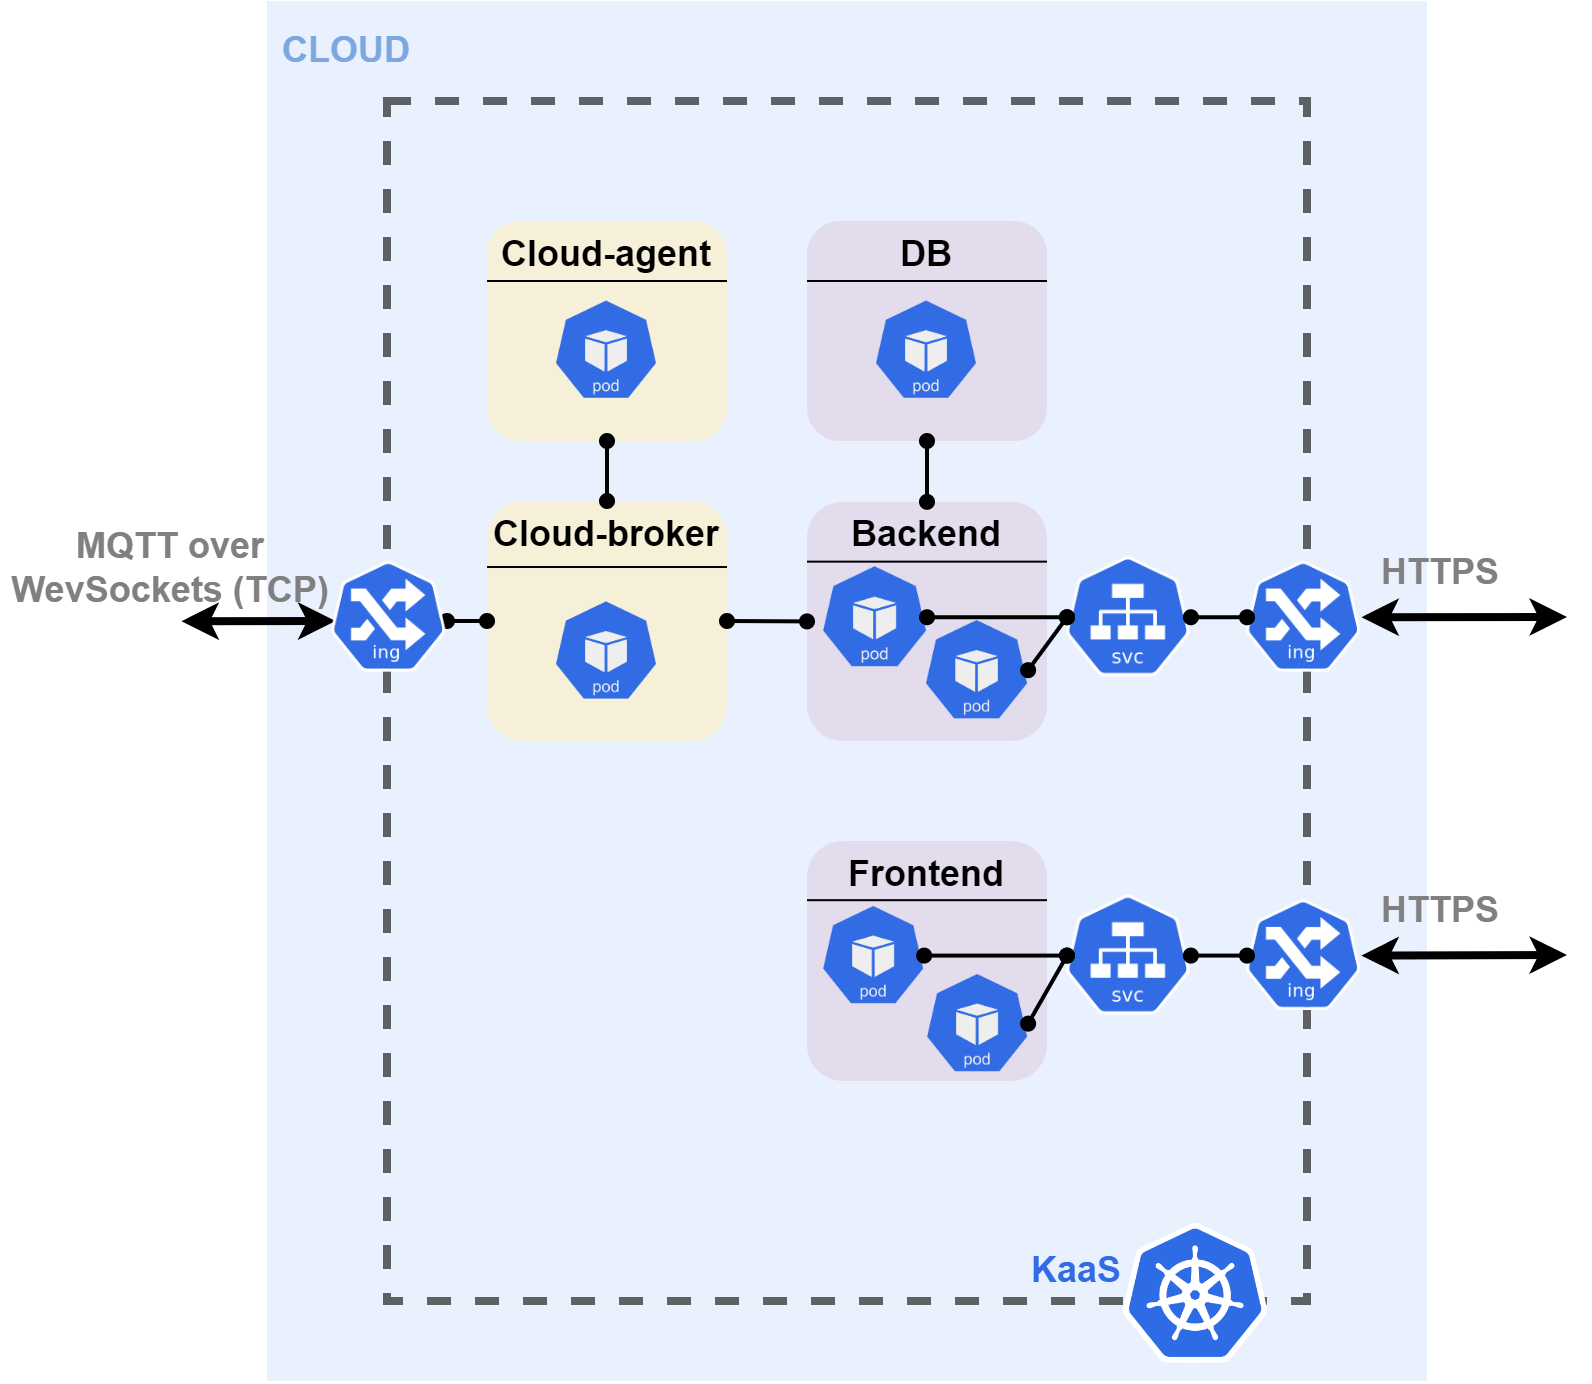
\includegraphics[width=0.8\textwidth]{pictures/cloud_services.png}
    \caption{ Cloud services system design }
    \label{fig:cloud_services}
\end{figure}

In this system design, three endpoints are exposed to external traffic, which originates from outside of the cluster. These include two HTTP/HTTPS endpoints for the Backend and Frontend and one WebSocket endpoint for MQTT messages that are sent to the cloud broker. HTTP/HTTPS traffic for frontend and backend is served through the use of ingress resources within the cluster. The traffic is forwarded via a reverse proxy(NGINX) to a Kubernetes service, which then distributes the request among the pods. The default ingress resource is designed to handle only HTTP/HTTPS requests and does not allow for any other protocol.

For the MQTT protocol, which is transported over TCP, a NodePort would typically be used to expose the service to the outside world. This maps pod ports to ports of the node in the cluster. However, some cloud providers do not permit the use of NodePorts, so a more flexible option was chosen, which involves bootstrapping the MQTT protocol over WebSockets and using ingress resources to handle external traffic coming to the cluster. This approach allows for the handling of MQTT traffic in a way that is compatible with the ingress resource and does not require the use of NodePorts.